\subsubsection{Parametertuning}
Dieser Paragraph beschäftigt sich mit der Ermittlung der maximal fahrbaren Geschwindigkeit bei Nutzung der entwickelten Bildverarbeitungs- und Regelungsstruktur. Durch die Auswertung verschiedener Messwerte soll der \glqq Flaschenhals\grqq\ gefunden und, wenn möglich, durch Parameteranpassung beseitigt werden.

Wichtige, noch anzupassende Parameter stellen dar:
\begin{itemize}
\item Die Frequenz, in der Bilder verarbeitet werden
\item Die Frequenz, mit der die Regelung stattfindet
\item Die Entfernung des Zielpunktes der Regelung vom Fahrzeug
\end{itemize}

Den Ausganspunkt für die folgenden Optimierungen bildet eine Geschwindigkeit von
\SI{0.1}{\metre\per\second}. Die Frequenz, mit welcher die Bilder verarbeitet werden wurde auf \SI{1}{\hertz} festgelegt, da die Extraktion der Linienpunkte eines Testbildes ca. \SI{0.5}{\second} benötigt. Die Frequenz der Regelung wurde initial auf \SI{20}{\hertz} festgelegt, da der Rechenaufwand für einen Regelungszyklus sehr gering ist. Eine noch höhere Regelfrequenz verspricht keinen Performancegewinn und läge schon nahe der maximalen Ansteuerfrequenz des Lenkservos sowie der Abtastrate der \gls{acr:imu} (jeweils \SI{50}{\hertz}).

Mithilfe dieser Einstellung absolvierte das Fahrzeug erfolgreich eine Runde im Testparcours. Wie in Abb.~\ref{fig:evaluation:riverflow:times_combined_1Hz_0_1m_s_over_piciter} zu sehen, benötigt ein Bild-Callback im Echtzeitbetrieb, d.h. bei mehrmaliger Ausführung erheblich weniger Zeit als beim einmaligen Messung anhand eines Testbildes. Die Verringerung der Bearbeitungsdauer \scl{t_{img}} von ca. \SI{500}{\milli\second} auf \SI{128}{\milli\second} (Median der in Abb.~\ref{fig:evaluation:riverflow:times_combined_1Hz_0_1m_s_over_piciter} dargestellten Daten) lässt sich unter anderem durch die Fahigkeit MATLABs, Funktionen bei wiederholter Ausführung im Hauptspeicher zu halten und somit schneller ausführen zu können, erklären. Eine signifikante Erhöhung der Bildfrequenz \scl{f_{img}} ist also möglich. Nimmt man die vom der Regelung und Posenaktualisierung, d.h. dem Odometrie-Callback  pro Sekunde benötigte Zeit \scl{t_{odom-per-sec}} als konstant an, lässt sich die theoretisch mögliche Bildfrequenz wie folgt berechnen:
\begin{subequations}
\begin{equation}
	T_{img} = t_{img}+t_{odom-per-sec}\cdot T_{img}
\end{equation}
%\begin{equation}
%	T_{img}\cdot(1-t_{odom-per-sec}) = t_{img}
%\end{equation}
\begin{equation}
	T_{img} = \frac{t_{img}}{1-t_{odom-per-sec}}
\end{equation}
\begin{equation}	
	f_{img} = \frac{1}{T_{img}}
\end{equation}
\end{subequations} 
Mit einer Bildbearbeitungszeit \(t_{img}=\SI{128}{\milli\second}\) sowie dem Zeitbedarf des Odometrie-Callbacks von \(t_{odom-per-sec}=\SI{262}{\milli\second\per\second}\) ergibt sich eine in der Theorie nutzbare Framerate von über \SI{5}{\hertz}. Mit dieser Bildfrequenz wurde eine weitere Testfahrt absolviert, in Abb. \ref{fig:evaluation:riverflow:times_pic_5Hz_0_2m_s_over_piciter} wird die bessere Nutzung der zur Verfügung stehenden Rechenzeit deutlich. Abbildung \ref{fig:evaluation:riverflow:times_pic_5Hz_0_2m_s_over_piciter} zeigt jedoch, dass die Periodendauer der Bildverarbeitung zwischen 2 Punkten oszilliert. Der erwartete zeitliche Abstand zweier konsekutiver Aufnahmen von \SI{200}{ms} wird häufig nicht erreicht, stattdessen befindet sich ein Abstand von \(2 \cdot \SI{200}{ms} = \SI{400}{ms}\) zwischen aufeinander folgenden Bildern. Dies führt zu dem Schluss, dass durch nicht vorhandene Pufferung Aufnahmen ausgelassen wurden.

\begin{figure}[ht] % [htb]
\centering
\subfloat[\SI{5}{\hertz}\label{fig:evaluation:riverflow:times_pic_5Hz_0_2m_s_over_piciter}]{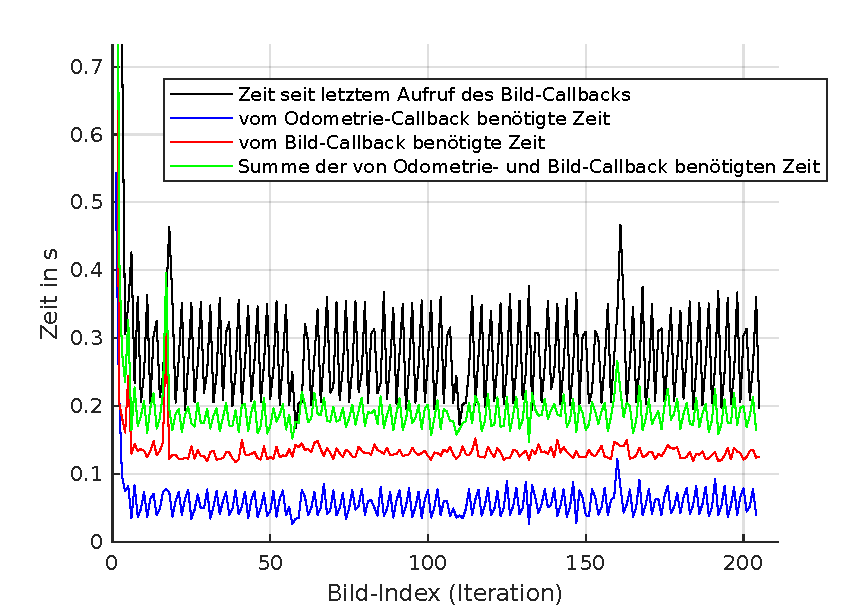
\includegraphics[width=0.45\textwidth]{evaluation_riverflow_times_combined_5Hz_0_2m_s_over_piciter}}
\qquad
\subfloat[\SI{4}{\hertz}\label{fig:evaluation:riverflow:times_pic_4Hz_0_2m_s_over_piciter}]{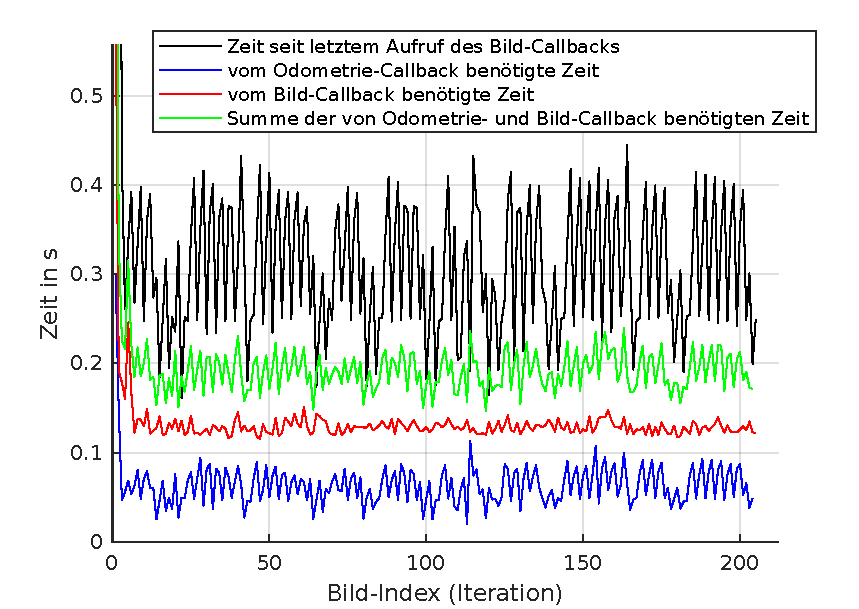
\includegraphics[width=0.45\textwidth]{evaluation_riverflow_times_combined_4Hz_0_2m_s_over_piciter}}
\qquad
\subfloat[\SI{3}{\hertz}\label{fig:evaluation:riverflow:times_pic_3Hz_0_2m_s_over_piciter}]{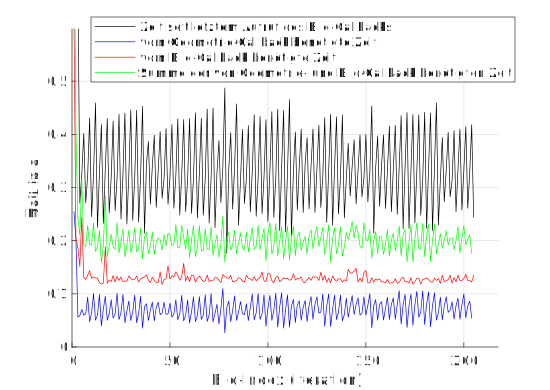
\includegraphics[width=0.45\textwidth]{evaluation_riverflow_times_combined_3Hz_0_2m_s_over_piciter}}
\subfloat[\SI{1}{\hertz}\label{fig:evaluation:riverflow:times_combined_1Hz_0_1m_s_over_piciter}]{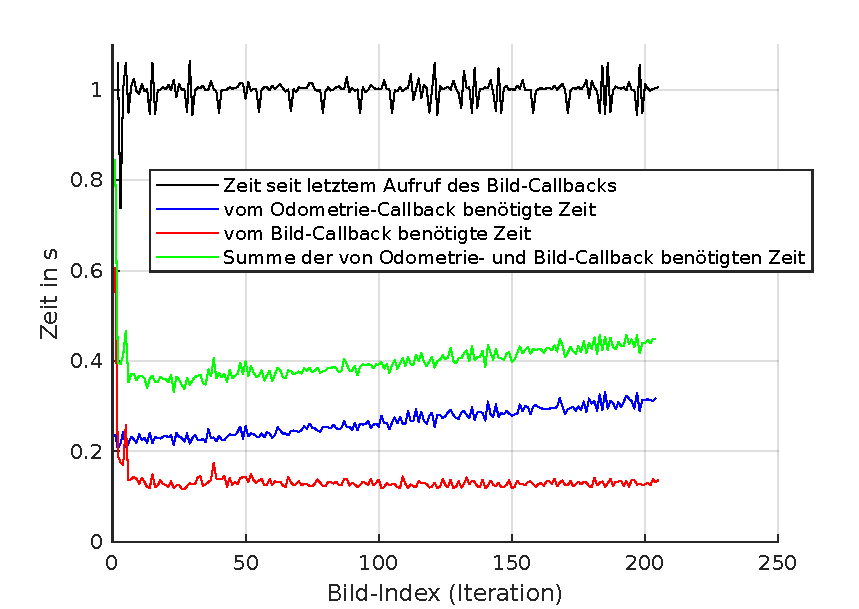
\includegraphics[width=0.45\textwidth]{evaluation_riverflow_times_combined_1Hz_0_1m_s_over_piciter}}
\caption{Zeitbedarf aller Fahrspurverfolgungskomponenten bei \SIlist{5;4;3;1}{\hertz} Bildfrequenz}
\end{figure}

Im folgenden wurde die Bildfrequenz zuerst auf 4 (s.Abb. \ref{fig:evaluation:riverflow:times_pic_4Hz_0_2m_s_over_piciter}), später auf \SI{3}{\hertz} verringert (s.Abb. \ref{fig:evaluation:riverflow:times_pic_3Hz_0_2m_s_over_piciter}). Erst jetzt konnte kein Springen der Periodendauer des Bild-Callbacks auf ein Vielfaches seines Erwartungswertes mehr festgestellt werden. Eine leichte Oszillation des zeitlichen Abstands zweier Aufnahmen ist auch in Abb. \ref{fig:evaluation:riverflow:times_pic_3Hz_0_2m_s_over_piciter} zu erkennen, jedoch beträgt der Mittelwert fast exakt die erwarteten \SI{333}{ms}. Die verbleibenden Unregelmäßigkeiten sind auf den Kamera-Node, welcher die Bilder aufnimmt und im entsprechenden Topic veröffentlicht, hervorgerufen werden (s. Abschnitt \ref{ssec:software_struktur:ros:nodes}). Abbildung \ref{fig:evaluation:riverflow:times_combined_3Hz_0_2m_s_pie_median} bzw. \ref{fig:evaluation:riverflow:times_combined_3Hz_0_2m_s_pie_mean} stellt nocheinmal die pro Bild mit Regelung,Bildverarbeitung,sonstigem Overhead\& im Leerlauf verbrachte Zeit einer gefahrenen Runde dar.

\begin{figure}[ht] % [htb]
	\centering
	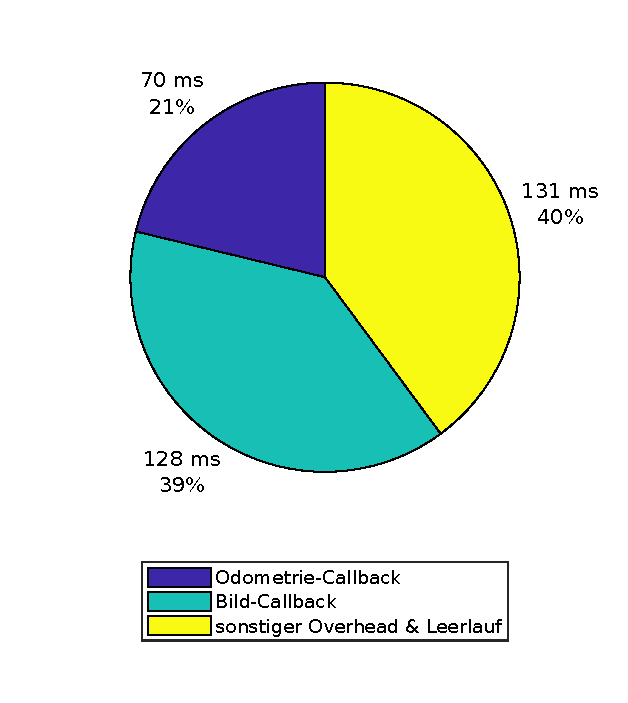
\includegraphics[width=0.7\textwidth]{evaluation_riverflow_times_combined_3Hz_0_2m_s_pie_median}
	\label{fig:evaluation:riverflow:times_combined_3Hz_0_2m_s_pie_median}
	\caption{Zeitbedarf aller Fahrspurverfolgungskomponenten bei \SI{3}{\hertz} Bildfrequenz; Median aller Messwerte einer Runde der Teststrecke}
\end{figure}

\begin{figure}[ht] % [htb]
	\centering
	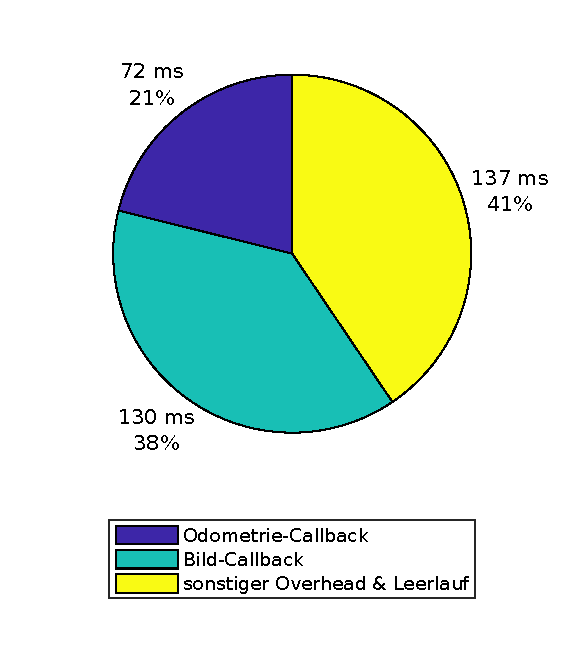
\includegraphics[width=0.7\textwidth]{evaluation_riverflow_times_combined_3Hz_0_2m_s_pie_mean}
	\label{fig:evaluation:riverflow:times_combined_3Hz_0_2m_s_pie_mean}
	\caption{Zeitbedarf aller Fahrspurverfolgungskomponenten bei \SI{3}{\hertz} Bildfrequenz; Mittelwert aller Messwerte einer Runde der Teststrecke}
\end{figure}

\paragraph{Dauer einzelner Komponenten der Bildverarbeitung}

\begin{figure}[ht] % [htb]
	\centering
	\subfloat[Boxplot ohne Startphase\label{fig:evaluation:riverflow:times_pic_3Hz_0_2m_s_boxplot}]{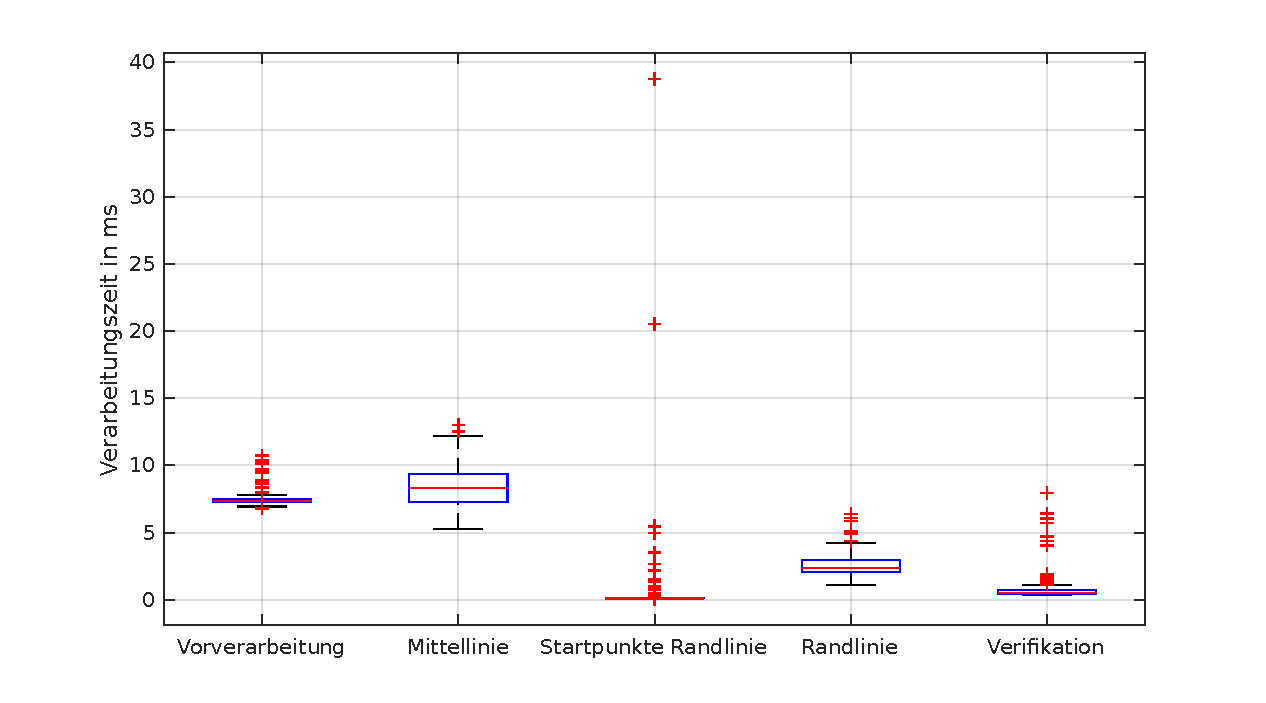
\includegraphics[width=0.7\textwidth]{evaluation_riverflow_times_pic_3Hz_0_2m_s_boxplot}}
	\qquad
	\subfloat[Boxplot ohne Startphase\label{fig:evaluation:riverflow:times_pic_3Hz_0_2m_s_boxplot_ros}]{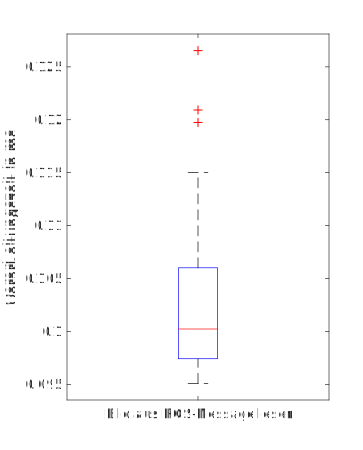
\includegraphics[width=0.2\textwidth]{evaluation_riverflow_times_pic_3Hz_0_2m_s_boxplot_ros}}
	\subfloat[Tortendiagramm; Median aller Messwerte einer Runde\label{fig:evaluation:riverflow:times_pic_3Hz_0_2m_s_pie_no_ros}]{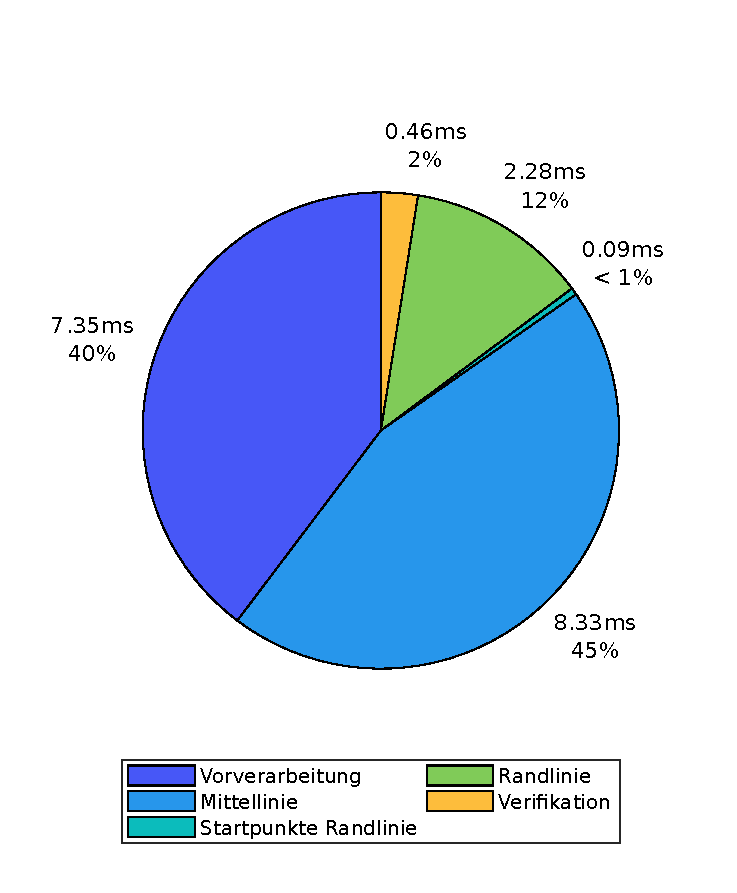
\includegraphics[width=0.45\textwidth]{evaluation_riverflow_times_pic_3Hz_0_2m_s_pie_no_ros}}
	\qquad
	\subfloat[Tortendiagramm; Median aller Messwerte einer Runde; mit Dekompression des Bildes\label{fig:evaluation:riverflow:times_pic_3Hz_0_2m_s_pie_with_ros}]{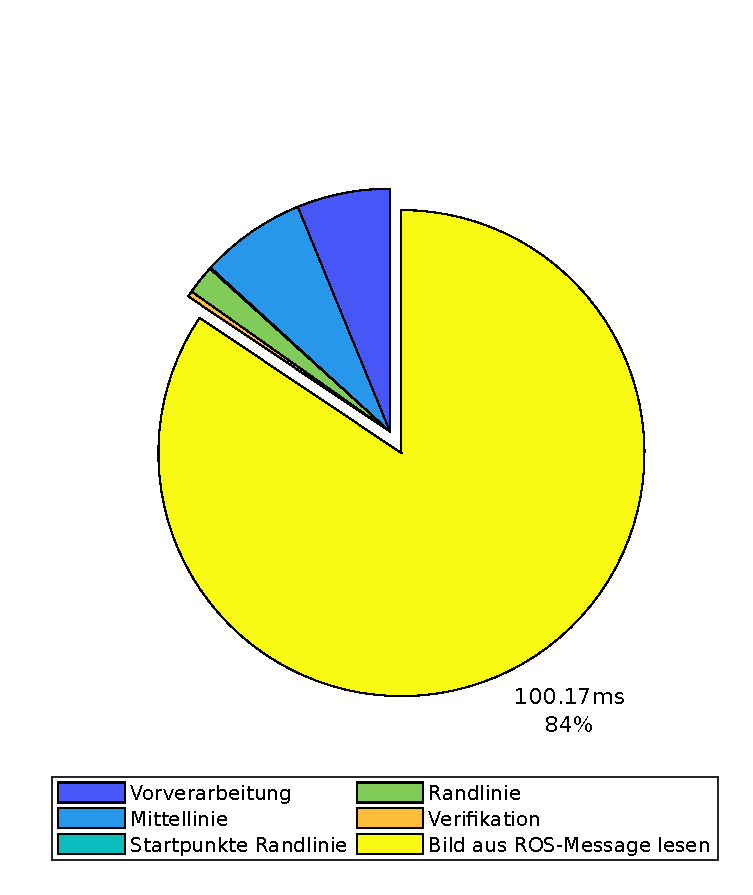
\includegraphics[width=0.45\textwidth]{evaluation_riverflow_times_pic_3Hz_0_2m_s_pie_with_ros}}
	\caption{Zeitbedarf aller Fahrspurerkennungskomponenten bei \SI{3}{\hertz} Bildfrequenz}
\end{figure}

\paragraph{Übertragungszeit}
